\documentclass[a4paper]{article}

\usepackage[portuguese]{babel}
\usepackage[utf8]{inputenc}
\usepackage[T1]{fontenc}
\usepackage{graphicx}
\usepackage{caption}
\usepackage{anysize}
\usepackage{amsmath}

\usepackage{hyperref}
\hypersetup{
	pdftitle = {CAD - TP2}
	,pdfauthor = {João Ferreira \& José Ribeiro Departamento de Engenharia Informática Universidade De Coimbra \texttt{jpbat@student.dei.uc.pt |  jbaia@student.dei.uc.pt}}
	,pdfborder = {0 0 0}
}

\title{Computação de Alto Desempenho - Trabalho Prático 2}
\author{João Ferreira \& José Ribeiro\\
		Departamento de Engenharia Informática\\
		Universidade de Coimbra\\
		\texttt{jpbat@student.dei.uc.pt | jbaia@student.dei.uc.pt}\\
		\texttt{2009113274 | 2008112181}}
\date{Junho 2013}

\marginsize{3.5cm}{3.5cm}{3cm}{3cm}

\begin{document}
\maketitle

\clearpage

\tableofcontents
\clearpage

\setlength{\parindent}{1cm}
\setlength{\parskip}{0.3cm}

\section{Introdução}
\indent \indent Tal como foi referido no relatório anterior, é cada vez mais díficil aumentar a frequência dos processadores, pelo que se verificou um aumento do número de processadores por computador. No entanto, como seria fácil de prever, também este aumento tem uma barreira, pelo que existiu a necessidade de apostar em computação distribuída.

Assim surge o conceito de \textit{cluster}, um aglomerado de computadores que estão ligados a um \textit{switch} de alta velocidade, o que lhes permite fazer computação distribuída através de, por exemplo, passagem de mensagens entre eles.

Neste contexto surge a biblioteca \textit{Message Passing Interface}, que nos foi apresentada pelo docente nas aulas teóricas e que vai ser por nós utilizada neste projecto.

Iremos detalhar o algoritmo utilizado, após o qual passaremos à análise dos resultados dos testes efectuados.
\clearpage

\section{Ambiente de Testes}
\indent \indent Os testes foram executados nos servidores disponibilizados pelo professor, sendo que pelo que nos foi possível constatar estas são as especificações técnicas de cada um deles:
\begin{description}
	\item [Processador] Intel(R) Xeon(R) CPU E5405 @ 2.00GHz, que possui 2 cores e 12MB de L2 Cache.
	\item [Memória RAM] 3.7GB.
	\item [Sistema Operativo] CentOS 6.3.
\end{description}

Ao longo do período de desenvolvimento fomo-nos deparando com alguns problemas no ambiente de testes; a maior parte deles causaram falhas silenciosas que demoraram, pela sua natureza, a serem detectadas.

O primeiro destes problemas foi não possuirmos espaço na nossa zona pessoal para conseguir guardar o ficheiro de output. Para o solucionar foi necessário que primeiro conseguissemos perceber que o erro não era causado por falha do envio de mensagens e, acima de tudo, que não era um erro de lógica no algoritmo, pelo que foi necessário fazer \textit{debug} da nossa solução, algo que não é de todo trivial num programa distribuído. Após termos descoberto a causa da escrita incompleta, resolvemos o problema recorrendo à directoria \texttt{/tmp/} do sistema, onde não existem restrições ao nível de permissões de escrita ou espaço.

Outro problema foi causado pelos próprios estudantes, quando por vezes se iniciavam \texttt{runs} sem que se verificasse se estava alguém a utilizar as máquinas. Para além disto nos levar a ter tempos errados de execução, causava falhas de segmentação, pois não teríamos disponível toda a memória de que precisávamos. Para resolver este problema utilizou-se o \texttt{htop} para que se pudesse controlar tanto os níveis de utilização dos \textit{CPU} das 9 máquinas, como os utilizadores que estariam a utilizar de modo a que se pudesse racionalizar o tempo exclusivo de processamento.

Um dos principais problemas que tivemos quando se tentou fazer \textit{fine tune} de alguns valores foram as consideráveis variações nos tempos de execução, algo que não faziamos ideia do porquê de acontecer. Eventualmente concluímos estar relacionado com o reescrever do ficheiro, que obrigava o sistema operativo a apagá-lo internamente; isto fazia com que o processo de remoção fosse contabilizado no tempo de execução. Assim, modificámos o ficheiro de \texttt{makefile} de forma a remover o ficheiro de \textit{output} anterior antes de executar, o que nos permitiu subtrair cerca de \textbf{2 segundos}.
\clearpage

\section{Abordagens}
\subsection{Generalidades}
\indent \indent Uma vez que no primeiro projecto criámos aquilo que achámos ser a melhor solução possível para resolver o problema, a nova abordagem consiste em correr a versão 1.0 do projecto em cada uma das máquinas, sendo que, em cada uma dessas máquinas, o processo de \textit{matching} se aplica às transacções que lhe correspondem (obtidas a partir do cálculo relativo ao seu offset).

Após isto, foi necessário fazer \textit{fine tune} a alguns valores, como por exemplo o tamanho ideal do \textit{buffer} de envio em cada uma das máquinas, ou qual a dimensão do \textit{batch} de transacções que garantia uma boa relação com o tamanho do \textit{buffer} e, ao mesmo tempo, minimizava o tempo perdido no \texttt{lock}. A maior parte deste \textit{fine-tune} ocorreu enquanto desconhecíamos o último problema mencionado na secção anterior, pelo que modificações bastante profundas no código não produziram (aparentemente, na altura) qualquer alteração no tempo obtido, uma vez que estes variavam cerca de 25\% em \textit{runs} consecutivos. Viemos mais tarde a descobrir que essas variações ocorriam entre a execução após um \texttt{make clean} e a consecutiva a essa, uma vez que fizemos a rotina limpar a pasta de \textit{output}. Chegámos ao valor ideal de 2500 transacções por \textit{thread}.

Durante todos os testes efectuados verificou-se com o auxílio de ferramentas como o \textit{htop}, se existiriam mais alunos a utilizar os servidores, e o nível de ocupação dos vários processadores das máquinas utilizadas, de modo a que houvesse certezas sobre a validade dos resultados.
\begin{figure}[h]
	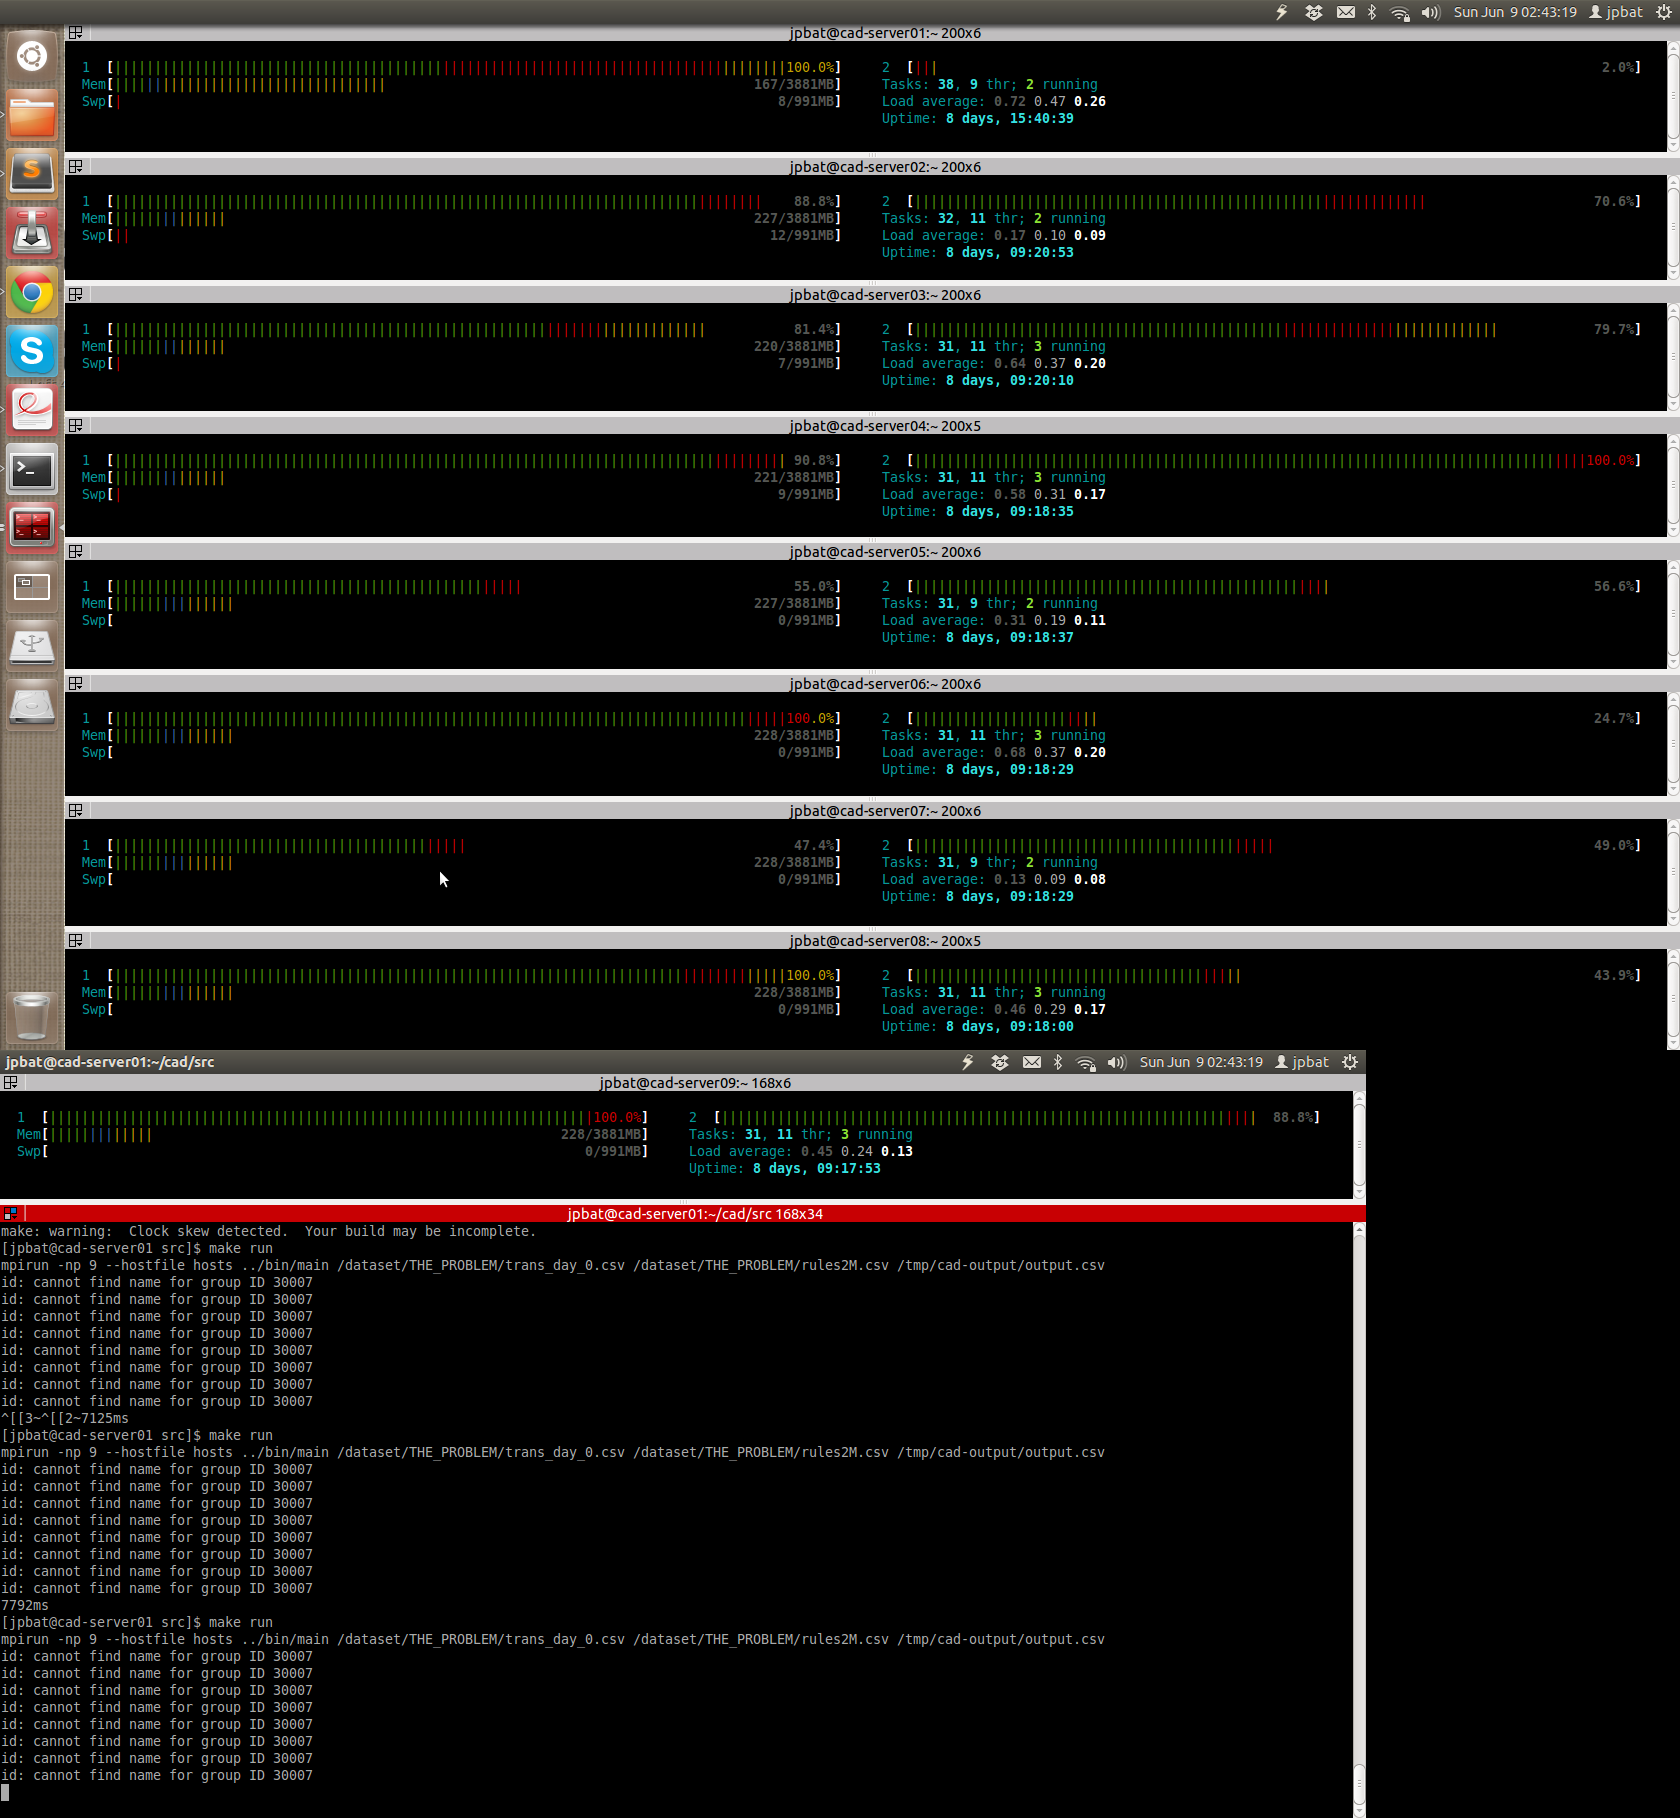
\includegraphics[keepaspectratio=true, width=0.4\textheight]{imgs/ocupacao.png}
	\caption{Monitorização do nível de ocupação dos CPUs.}
\end{figure}

\subsection{Arquitectura}
O algoritmo consiste na utilização de um nó \texttt{master} que recebe todos os resultados por parte dos seus \texttt{slaves} e que os escreve para disco.

Todos os nós \texttt{slave} calculam quais os índices de início e de fim das transacções que lhe são correspondentes a partir do seu \texttt{MPI rank}. Após isso, colocam esses índices na fila e correm as suas threads de forma a que estas obtenham trabalho e processem as transacções. Tal como no trabalho anterior, cada thread possui um buffer próprio para onde escreve sem ficar bloqueado em \textit{locks}. No entanto, este \textit{buffer}, ao contrário do projecto anterior, não contém as strings ASCII já representantes da forma final que ficaria no ficheiro, mas sim os pares \texttt{transaction\_id}/classificação. Fazemo-lo desta forma para minimizar o tráfego na rede.

Assim que este buffer se encontra completo, é necessário enviá-lo ao \texttt{master node} de forma a que este os escreva para ficheiro. Tal é feito recorrendo a um \texttt{MPI\_Send}. Usámos a chamada síncrona uma vez que necessitávamos de garantir que existia memória suficiente, enquanto que a versão \textit{buffered} consumia bastante memória (uma vez que os pedidos iam acumulando dada a velocidade de processamento do \texttt{master node} ser limitada).

O \texttt{master node} encontra-se bloqueado na recepção dos resultados e processa-a, transformando os pares de inteiros em representações ASCII em memória, após o qual as escreve para disco num único \texttt{write}.

\subsubsection{V1.0}
\indent \indent Numa primeira versão, utilizámos \texttt{MPI\_Recv} do lado do \texttt{master}, de forma a receber sincronamente e processar todos os dados. Esta era a abordagem mais simples; no entanto, a recepção consome tempo que poderia ser usado no processamento. Assim procedeu-se à segunda abordagem.

\subsubsection{V2.0}
\indent \indent A segunda versão consistiu em utilizar \texttt{MPI\_Irecv}, versão não bloqueante da recepção de dados. Isto permite que a recepção de dados seja feita assincronamente, o que permite o processamento e escrita para ficheiros em simultâneo no \texttt{master}, pelo que este apenas bloqueia na ausência de trabalho.

\clearpage


\section{Resultados}
\indent \indent No primeiro projecto conseguiu-se atingir uma performance de 200000 transacções por segundo numa máquina com seis cores, sendo que nesta a performance do nosso melhor algoritmo não foi além de X. Existem várias razões que podem justificar estes resultados. Neste segundo projecto as nove máquinas a que temos acesso estão a ser virtualizadas, pelo que mesmo cada uma delas tendo o seu próprio sistema de ficheiros, nada garante que fisicamente os ficheiros não estão no mesmo disco rígido, havendo assim um possível \textit{bottleneck} nos acessos a disco. Outra razão que pode explicar estes resultados é o facto de a máquina master ser \textit{single threaded}, pelo que é perdido muito tempo em operações de \texttt{MPI IO}. Por fim o facto de haver alguma, ainda que pouca, latência nas comunicações feitas pela rede pode também ajudar a explicar a performance da nossa solução.

\begin{figure}[h]
	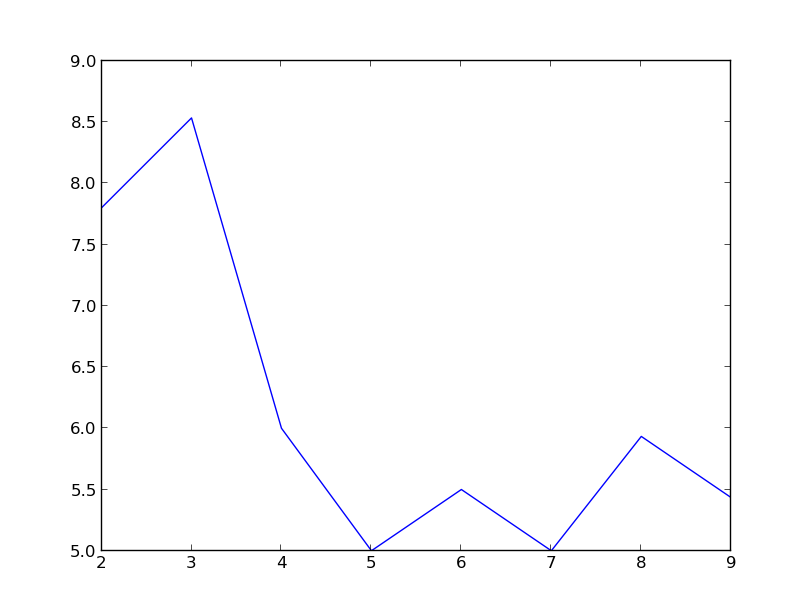
\includegraphics[keepaspectratio=true, width=0.4\textheight]{imgs/scalabilityv1.png}
	\caption{V1 - Tempo de execução em função do número de nós.}
\end{figure}
\begin{figure}[h]
	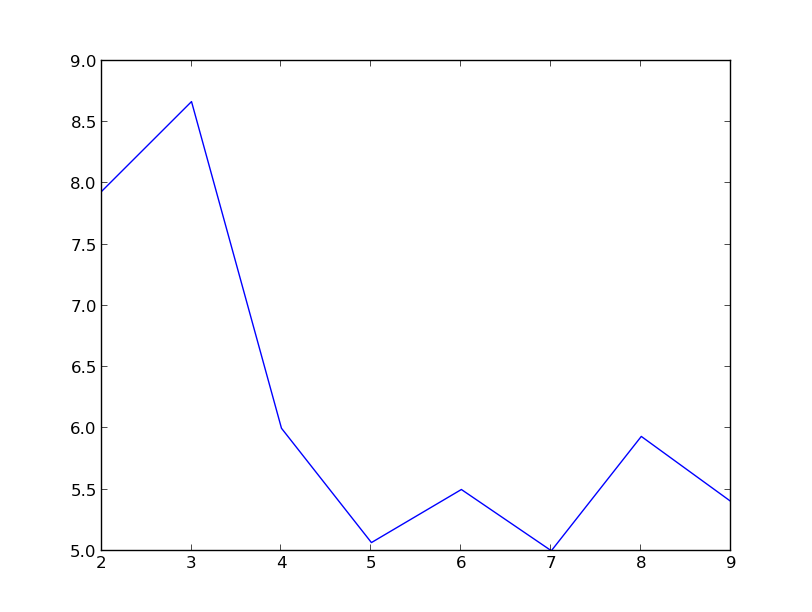
\includegraphics[keepaspectratio=true, width=0.4\textheight]{imgs/scalabilityv2.png}
	\caption{V2 - Tempo de execução em função do número de nós.}
\end{figure}
\clearpage


\section{Conclusão}
\indent \indent Com o fim do projecto, já depois de termos reflectido sobre todos os dados que foram recolhidos, chega por fim a altura em que se tiram conclusões.

Com este projecto aprendemos que o mundo da virtualização de máquinas tem os seus pontos positivos e os seus pontos negativos. É realmente fácil ``criar'' máquinas mas por vezes é pago a peso de ouro o custo dos acessos ao hardware limitado.

Além disto aprendemos que ter um supercomputador não significa necessariamente ter um computador com um poder de processamento gigantesco, mas que pode significar também pegar em meia dúzia de computadores francamente mais fracos e ligá-los em rede. Existem claramente vantagens em termos financeiros, sendo que por outro lado é algo mais díficil de programar e sobretudo fazer debug numa arquitectura distribuída.
\clearpage
\end{document}
